\documentclass[10pt,a4paper]{article}
\usepackage[utf8]{inputenc}
\usepackage[english]{babel}
\usepackage{lmodern}
\usepackage[left=2cm,
			right=2cm,
			top=1.5cm,
			bottom=2cm,
			headheight=3ex,
			headsep=2ex]{geometry}

\usepackage[obm]{zeusproblems}
\usepackage{zeusall}

\setlength\parindent{0pt}

\def\primaryLanguage{en}

\pagestyle{empty}

%\renewcommand{\playerA}[1]{Guilherme}
%\renewcommand{\playerB}[1]{Zeus}

\begin{document}

\begin{center}
\begin{minipage}[t][2cm][t]{2cm}
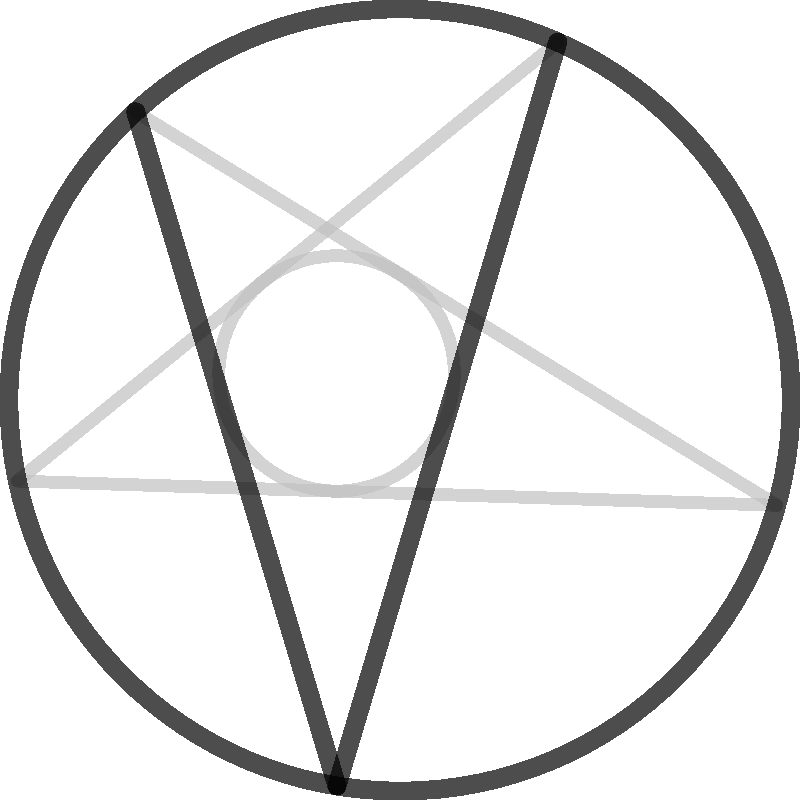
\includegraphics[width=2cm]{logo.pdf}
\end{minipage} \hspace{3em}
\raisebox{1.25cm}{
\begin{minipage}[t][1cm][t]{8.5cm}
\begin{center}
	\bfseries 19$^\text{th}$ Olympic Revenge
	
	23$^\text{rd}$ Olympic Week -- Natal, RN
	
	January 30 and 31, 2020
\end{center}
\end{minipage} \hspace{3em}}
\end{center}

\hrule
\begin{itemize}
	\item Don't write more than one question per sheet. \setlength\itemsep{0.1em} 
	\item Write your name in every sheet of paper you use.
\end{itemize}
\hrule\hspace{0.5em}

\problem{math/brazil/vinganca/2020/banco/7}
\problem{math/brazil/vinganca/2020/banco/3}
\problem{math/brazil/vinganca/2020/banco/1}
\problem{math/brazil/vinganca/2020/banco/8}
\problem{math/brazil/vinganca/2020/banco/6.2}

\vfill

{\itshape Linguagem: English \hfill Duration: 5 hours.}

{\hfill \itshape Each problem is worth 7 points.}


\hspace{1em}

\hrule

\end{document}
